\documentclass{article}
\usepackage[utf8]{inputenc}
\usepackage{graphicx}
\graphicspath{ {./images/} }

\title{Agent-based models of non-pharmaceutical interventions for epidemic control}
\author{Robert Brian Milligan and Supervised by Julian Garcia Gallego \& Buser Say}
\date{7 July 2022}


\begin{document}

\tableofcontents

\maketitle

\section{Introduction}
This paper investigates the modificaiton of an existing model diease spread produced by Ryan McGee and used a part of various peer reviewed research articles. I have looked at applying the model to the situation of COVID-19 in childcare and involves creating both a non stategic and strategic behavoioural models. The Behaviour relates to compliance to various actions the agent can choose to do such as doing an additional COVID rapid antigent test if they have symtoms of the virus.

\section{Description of Model}
\subsection{Description of purpose of the network in the model}
The model has two structures agents can be arranged in , one which uses a one single connected network designed to simulate a workplace, the other has a group of age segregated connected networks as well as small networks each agent is a part of that represents the household they are in. These large networks are made up of a number of cohorts which are loosely connected and each of these has a number of subgroups which are highly connected.

The network is set up before the simulation begins and does not change throughout the simulations run. 80\% of transmission spread between agents occurs along the edges connecting them, while 20\% of transmission is at  random

Each day agents will be asked to do a test if their day has come up on a surveillance testing schedule, they show symptoms or have been contacted that they are a close contact.

During the day agents can spread the contagion to each other and can progress though the stages of the disease if they have it. They additionally have the choice to participate in contact tracing.

Agents will also be asked to isolate for one of six reasons. They or a group member develop a symptomatic case, returns a positive test or is told they are a close contact though using contact tracing

These systems can effectively be disabled by overriding the compliance for them to be a large negative number, for example compliance with contact tracing can be set to -10 to disable the use of that system.

The model has a variety of limitations including 
\begin{itemize}
\item Having all agents always test on the same day, so if semiweekly is chosen, all agents will be asked to test on Monday and Thursday
\item the network itself is unchanging, but this is not necessarily bad
\end{itemize}

\begin{figure}
  \centering
      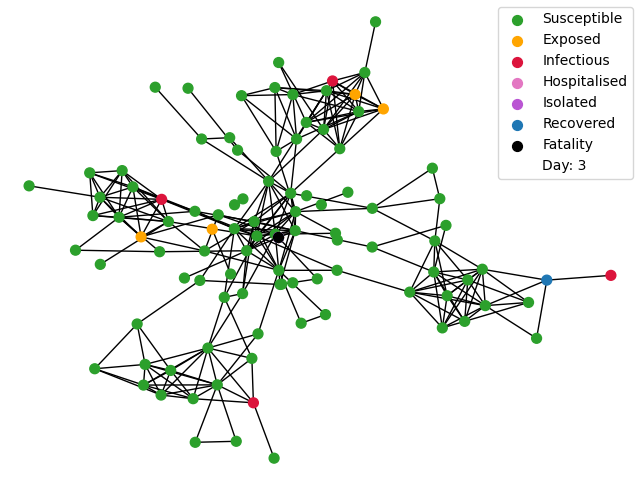
\includegraphics[width=\textwidth]{network}
  \caption{An Example Netowrk}
\end{figure}


Example of the network of 100 agents
To simulate the childcare scenario they are split into 5 groups of about 20 agents each with high connectivity inside the group and low connectivity between the groups 
The agents current state is shown by the nodes colour and the edges are that agents close contacts which the disease can spread easiest though the population


\subsection{Description of Model Parameters}
The Current Modifications of the model relate to allowing 10 of the Model Parameters that relate to Compliance to be dynamically updated each day dependent on a given rule. The 5 most relevent of these being.
\begin{itemize}
\item TESTING\_COMPLIANCE\_RATE\_SYMPTOMATIC (what proportion of agents take a test immediately as a result of having symptoms)
\item TESTING\_COMPLIANCE\_RATE\_RANDOM  (what proportion of agents will do surveillance)
\item ISOLATION\_COMPLIANCE\_RATE\_SYMPTOMATIC\_INDIVIDUAL (what proportion of agents will isolate given they have a symptomatic case)
\item ISOLATION\_COMPLIANCE\_RATE\_POSITIVE\_INDIVIDUAL (what proportion of agents will isolate given a positive result from a test)
\item ISOLATION\_COMPLIANCE\_RATE\_POSITIVE\_GROUPMATE (what proportion of agents in a group isolate given one of them has a positive result from a test)
\end{itemize}

A simple model might only use a few of these compliance parameters such as  and is how the parameters work in the base model
\begin{itemize}
\item TESTING\_COMPLIANCE\_RATE\_SYMPTOMATIC = 0.5\
\item TESTING\_COMPLIANCE\_RATE\_RANDOM = 0.5
\item ISOLATION\_COMPLIANCE\_RATE\_POSITIVE\_INDIVIDUAL =1
\end{itemize}


\subsection{Description of Compliance In the Model}
Compliance can be set a variety of ways in the modified model but in this paper 3 are used
\begin{itemize}
\item The default setting where agents are given an inital value for compliance and is unchanging e.g. 50\% are set to comply and will always do so
\item The non stategic model where agents are given an inital compliance and can become more compliant depending on the network situation , their local situation or a mix
\item The stategic model where agents utilise knowledge of the amount of agents in the network who will comply to make a decision to comply or not
\end{itemize}



\section{Childcare Model and Benchmark Tests}

\begin{itemize}

\item Parameter justification
\item test false negative rate 0.36 https://www.abc.net.au/news/2022-02-05/staff-children-preschool-childcare-protected-covid-national-plan/100805610
\item R0 mean of Omicron is 9.5, delta is 5.4  https://www1.racgp.org.au/newsgp/clinical/what-to-expect-from-a-third-omicron-wave-in-austra https://academic.oup.com/jtm/article/29/3/taac037/6545354
\item base compliance for behaviour is set t 0.5
\item 100 agents in model split into 5 groups with high interconnectedness within the group and low connections between groups

\item compliance increases for 2 actions,  symtomatic test and regular interva survillencel tests
\item The cost of compliance is is fixed and there is a reward based on if connecting agents are isolated, hospitalised or a fatality

\item from looking at early results since only 2-3 tests a week there is a delay and the higher the r0 the fewer chances they can have to change their mind about compliance 

\item the R0 of 9.5 or 5.4 may be too high as it assumes children spread the disease at the same rate as the general population as well as all disease spread occuring in childcare which it probably is not. Therefore 2 other R0 cases of 3 and 2 are used as they may more accuratley capture a real world scenario where not all transmision is though the 1 childcare setting
\end{itemize}

\begin{figure}
  \centering
      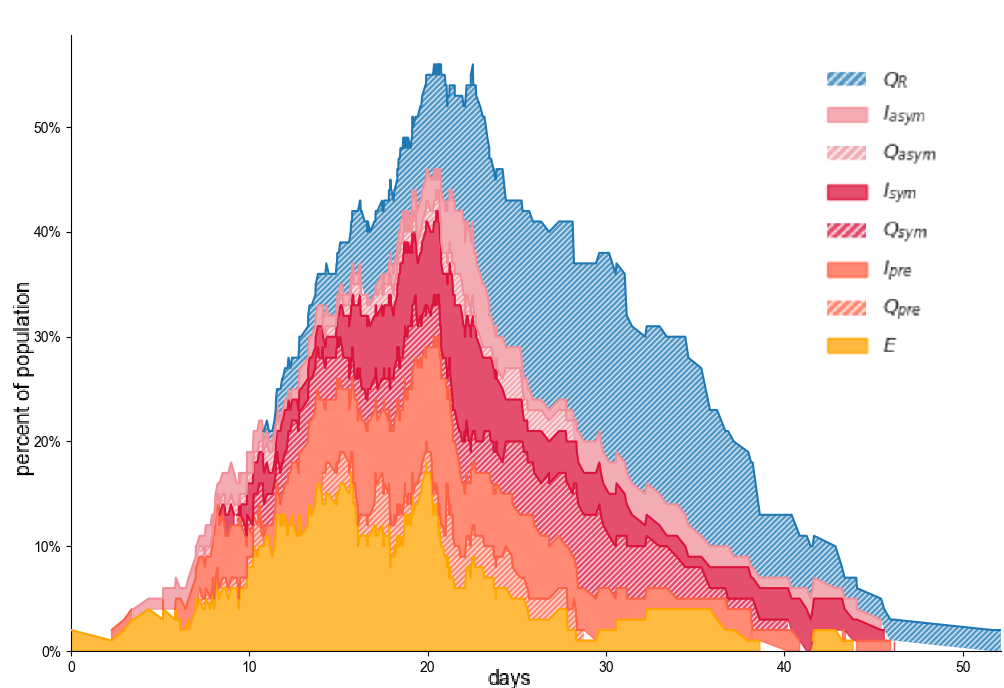
\includegraphics[width=\textwidth]{Figure3}
      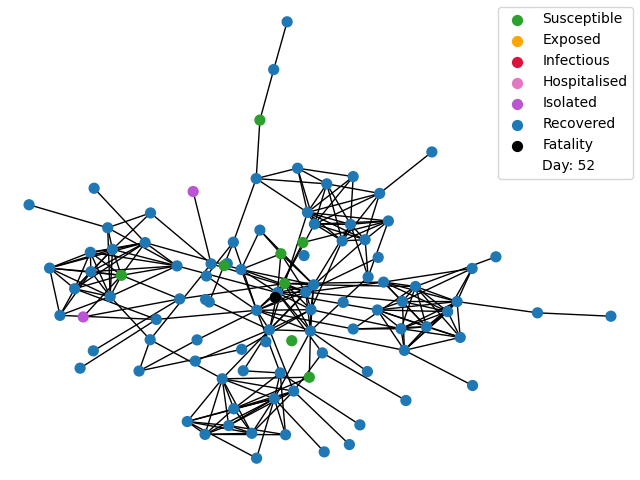
\includegraphics[width=\textwidth]{Figure3Net}
  \caption{Benchmark Run with Unchanging Compliance at 50\% for regular twice weekly survilence testing and testing if symtomatic with the resulting final network. 92 of the 100 agents received the infection}
\end{figure}


\section{Non-Strategic Model}
We have a fixed cost of compliance to an action and varying factors that can raise it. A mix of global and local behavioural factors can be added to make an agent more compliant. In the current build these are the known positive cases in the network in the past 14 days. The proportion of contact agents (those which share an edge) which are a fatality, hospitalised or in isolation. These values are taken away from the base cost and if the result is lower from a specified value the agent will be compliant to that action, otherwise they are not

For a simple example we have a situation for this central agent 


\begin{figure}
  \centering
      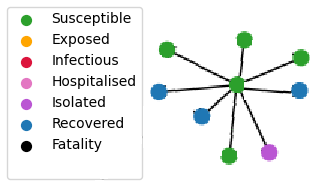
\includegraphics[width =150pt]{basicnet}
  \caption{An Example Simplified Network}
\end{figure}


TESTING\_COMPLIANCE\_RATE\_SYMPTOMATIC                  = 0.5
TESTING\_COMPLIANCE\_RATE\_RANDOM                       = 0.5

14 day positive test rate for network = 0.02 = 2%
This agent’s base aptitude +0.30 which can range (-0.5,0.5)
Base cost = 0.5
Compliance = 0.5 – (5 * 1/10) – (4*0.02) + 0.3 = 0.22
In this case the agent is compliant
will test if they develop a symptomatic case immediately
will do surveillance testing 
if the neighbouring agent that entered hospital returns a positive test, our agent will enter isolation

the reward for agents can be based on a mix of both a local and global network situation as in the example runs

Of the 10 possible compliance parameters built into the existing mode, 4 are used these are,
•	immediately testing if the agent has a symptomatic case
•	using regular surveillance testing
•	isolating if a positive test is returned


\begin{figure}
  \centering
      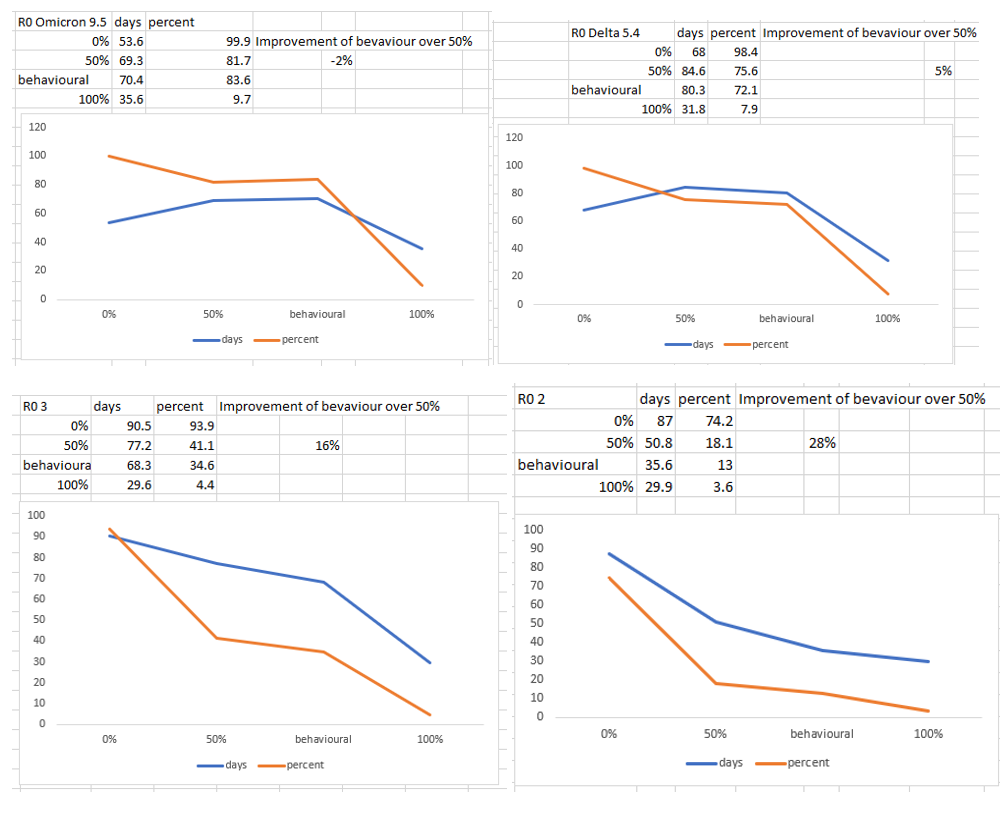
\includegraphics[width=\textwidth]{basicgraph}
  \caption{Test Results of a non strategic model}
\end{figure}



\section{Analysis of Testing Compliance}

On average, what percentage of the population caught the contagion
On average, how many days did it take for the outbreak to stop with 0 active cases

We can analyse compliance by comparing the effect varying levels have on the length a contagion actively spreads and what proportion of the population becomes infected. Firstly a baseline can be set to explore the parameter space, then further tests done to see the effect having compliance change as a result of the current known spread of the contagion in the network.


Over 4 different R0 virus base reproduction rate was the model run with, over the different R0 levels the reducion in total cases reduced from a -2\% improvement with an R0 of 9.5 to a 28\% improvement with an R0 of 2. This is probably due to one of the aspects the model relating to the 14 day known positive cases recorded. With a low R0 in the system there are more chances for agents to test themselves before they pass on the disease and these reported cases incentivise even more agents to do symptomatic and surveillance testing. With extremely high R0 numbers it is observed that the non-strategic behavioural model has little effect on the total number infected. Across all cases it can be seen that the amount of time the simulation runs for is tied with how many agents get infected. Both the static values of compliance and non-strategic behavioural model follow this trend. 



\section{Strategic Model}
The view of benefit and cost can be grouped into 3 categories.
There is a level at which people will not contribute as they find the act pointless as they know near no agents  will comply 
\begin{itemize}
\item1. Global Situation of the model e.g. changes over time but is idential across all agents
e.g. number of active cases or rate of change in spread rate , could place 2 infections in first week and compare each week to the last week, rate of change week on week
[0,0,0,0,0,0,2]  if the next week 4 cases are spread, the rate would be 2
\item2. Structural Layout of the model, identical over time but varies between each agents
e.g. number of close contacts or number of agents one can reach in 1 step , or could be 2 steps, the more agents one is in contact with the greater the benefit 
\item3. Structual Situation of the model, changes over time and varies for each agent
e.g. number of close contacts in a particular state or group of states like hospitalised, fatality, isolated etc, if a close contact is in one of those states the benefit to compliance is greater
\end{itemize}

for the following tests these can be used to create a personal benefit for each agent 

it could be possible to use of a mix of these siutaitons and in real life that may be the case with peoples decision making process


Structural layout of the network, for example number of close contacts an agent has 

global situation for example the number of reported cases in the last 2 weeks , the number of actual cases in the last 2 weeks, the growth of the disease spread rate

local situation for example the number of neighbouring agents that are a fatality, hospitalised or isolated


benefit depends on change on rate of disease , number of agents around you that are hospitalised, fatality or isolated

one model is exclusivley global, one is excluisley local


number of infections of those connected to me, 1 or 2 degrees , that are exposed or infectious

number of infections globally



agents will know the total percent of agents that are compliant and use that to work out how compliant they are

one universal curve for compliance , would this mean it has to be based off global factors ?

do I actually need to mathimatically work out a curve and its intecepts 

every day am I updating this curve? , can agents move to exactly where they want, or is it a slow process, they can only move X amount every day?, a limited amount makes sense as that would match the curves in other papers like thomas?
Or would you see where the maxima is on that day and instantly assign the end that value?

come up with a equation (payoff function), x parameter to produce a curve like in the papers
parameters go in , map plot, make it a notebook

does it change based on rate of change or on number of cases - if its global every curve would be the same
if its local every curve is different for each agent

notebook

how do curves change with infection numbers/rate

keep adding to latex doc.

once its a good function integrate it 

Redo table of content
Childcare first introduces compliance
Describe the model
 
When you comply you pay a cost

Growth of disease rate



\section{Results}

\section{Discussion}

\section{Conclusion}

\newpage
\appendix

\section{Appendix Section}

Removed parameter section
\begin{itemize}
\item TRACING\_COMPLIANCE\_RATE (what proportion of agents comply with contact tracing)
\item ISOLATION\_COMPLIANCE\_RATE\_POSITIVE\_CONTACT (what proportion of agents isolate given they are a close contact) 

\item TESTING\_COMPLIANCE\_RATE\_TRACED (what proportion of agents take a test immediately as a result of being informed they are a close contact)


\item ISOLATION\_COMPLIANCE\_RATE\_SYMPTOMATIC\_GROUPMATE (what proportion of agents will isolate given one of their group mates has a symptomatic case)

\item ISOLATION\_COMPLIANCE\_RATE\_POSITIVE\_CONTACTGROUPMATE (what proportion of agents in a group isolate given one of them is a close contact)
\end{itemize}

\end{document}
